%%% LaTeX Template: Designer's CV
%%%
%%% Source: http://www.howtotex.com/
%%% Feel free to distribute this template, but please keep the referal to HowToTeX.com.
%%% Date: March 2012


%%%%%%%%%%%%%%%%%%%%%%%%%%%%%%%%%%%%%
% Document properties and packages
%%%%%%%%%%%%%%%%%%%%%%%%%%%%%%%%%%%%%
\documentclass[a4paper,12pt,final]{memoir}

% misc
\renewcommand{\familydefault}{bch}	% font
\pagestyle{empty}					% no pagenumbering
\setlength{\parindent}{0pt}			% no paragraph indentation


% required packages (add your own)
\usepackage{flowfram}										% column layout
\usepackage[top=1cm,left=1cm,right=1cm,bottom=1cm]{geometry}% margins
\usepackage{graphicx}										% figures
\usepackage{url}											% URLs
\usepackage[usenames,dvipsnames]{xcolor}					% color
\usepackage{multicol}										% columns env.
	\setlength{\multicolsep}{0pt}
\usepackage{paralist}										% compact lists
\usepackage{tikz}
\usepackage{enumitem}
\usepackage[utf8]{inputenc}

%%%%%%%%%%%%%%%%%%%%%%%%%%%%%%%%%%%%%
% Create column layout
%%%%%%%%%%%%%%%%%%%%%%%%%%%%%%%%%%%%%
% define length commands
\setlength{\vcolumnsep}{\baselineskip}
\setlength{\columnsep}{\vcolumnsep}

% frame setup (flowfram package)
% left frame
\newflowframe{0.2\textwidth}{\textheight}{0pt}{0pt}[left]
	\newlength{\LeftMainSep}
	\setlength{\LeftMainSep}{0.2\textwidth}
	\addtolength{\LeftMainSep}{1\columnsep}
 
% small static frame for the vertical line
\newstaticframe{1.5pt}{\textheight}{\LeftMainSep}{0pt}
 
% content of the static frame
\begin{staticcontents}{1}
\hfill
\tikz{%
	\draw[loosely dotted,color=RoyalBlue,line width=1.5pt,yshift=0]
	(0,0) -- (0,\textheight);}%
\hfill\mbox{}
\end{staticcontents}
 
% right frame
\addtolength{\LeftMainSep}{1.5pt}
\addtolength{\LeftMainSep}{1\columnsep}
\newflowframe{0.7\textwidth}{\textheight}{\LeftMainSep}{0pt}[main01]


%%%%%%%%%%%%%%%%%%%%%%%%%%%%%%%%%%%%%
% define macros (for convience)
%%%%%%%%%%%%%%%%%%%%%%%%%%%%%%%%%%%%%
\newcommand{\Sep}{\vspace{1.5em}}
\newcommand{\SmallSep}{\vspace{0.5em}}

\newenvironment{AboutMe}
	{\ignorespaces\textbf{\color{RoyalBlue} Acerca de mi}}
	{\Sep\ignorespacesafterend}
	
\newcommand{\CVSection}[1]
	{\Large\textbf{#1}\par
	\SmallSep\normalsize\normalfont}

\newcommand{\CVItem}[1]
	{\textbf{\color{RoyalBlue} #1}}


%%%%%%%%%%%%%%%%%%%%%%%%%%%%%%%%%%%%%
% Begin document
%%%%%%%%%%%%%%%%%%%%%%%%%%%%%%%%%%%%%
\begin{document}

% Left frame
%%%%%%%%%%%%%%%%%%%%
\begin{figure}
	\hfill
	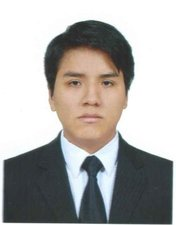
\includegraphics[width=0.6\columnwidth]{profile}
	\vspace{-7cm}
\end{figure}

\begin{flushright}\small
	Javier Huaman Adama \\
	\url{javier.adama@gmail}  \\
	(+51) 950450833
	\Sep
	\textbf{Dirección} \\
	Calle 3 de Mayo \\ % Address 1
	Mz. A Lt. 8 Urb. El Bosque \\ % Address 2
	Ate - Lima \\ % Address 3
\end{flushright}\normalsize
\framebreak


% Right frame
%%%%%%%%%%%%%%%%%%%%
\Huge\bfseries {\color{RoyalBlue} Javier Huaman Adama} \\
\Large\bfseries  Téc. Computación e Infórmatica \\

\normalsize\normalfont

% About me
\begin{AboutMe}
Soy proactivo, responsable, puntual y flexible a los cambios también me desenvuelvo mejor trabajando en grupo, me gusta formar parte de un ambiente laboral saludable. Me interesa trabajar en todo lo orientado al desarrollo de software (programación, prueba, despliegue e implementación).
\end{AboutMe}

% Education
\CVSection{Educación}
\CVItem{2017 - Actualidad, UPC}\\
Ingeniería de Sistemas
\SmallSep

\CVItem{2013 - 2015, CIBERTEC}\\
Técnico de Computación e Infórmatica
\SmallSep

\CVItem{2007 - 2012, Niño Jesús de Praga}\\
Secundaria completo.
\Sep

% Experience
\CVSection{Experiencia}
\CVItem{Mayo 2018 - Actualidad, Analista Programador, Consorcio Fabrica de Software}\\
- Implementación de Comprobantes de Pago Fisicos - SUNAT. Tecnologia usadas:\\
Java: Java EE, JSP, JPA, Git; Gradle; WEBLOGIC; Informix; Jquery/CSS/Html/Bootstrap.\\\\
- Implementación de Gestor de Operadores OSE - SUNAT. Tecnologia usadas:\\
Java: Java EE, JSP; JPA, Git, Gradle; WEBLOGIC; Informix; Jquery/CSS/HTML/Bootstrap.
\SmallSep

\CVItem{Mayo 2017 - Marzo 2018, Analista Programador, SYNOPSIS}\\
- Rediseño y migración del sistema Telebanking - Scotiabank. Tecnologia usadas:\\
Java: Spring MVC 4, Spring Security, Thymeleaf; Git; Gradle; AS400; WAS(WebSphere Liberty Profile); Hazelcast; SQLServer; Jquery/CSS/Html; JUnit.\\\\
- Diseño e implementación de la funcionalidad de Clave Digital para el uso en nuevos clientes como también la actualización de procesos transaccionales (Pagos, Transferencias y actualización de datos) para que utilicen dicha funcionalidad para la plataforma web de Scotia en Linea - Scotiabank. Tecnologia usadas:\\
Java: JavaEE, JSP; Jquery/CSS/HTML; DB2; AS400;Gradle;JUnit.\\\\
- Diseño e implementación de la funcionalidad Clave Digital a nivel de aplicaciones móviles para Scotia en Linea - Scotiabank. Tecnologia usadas:\\
Para la capa servicio: Java: JavaEE, EJB; Maven Multimódulo;DB2; AS400; JUnit.\\
Para aplicación móvil; Android: ButterKnife, MaterialDesign;SOAP/REST.
\SmallSep

\clearpage

\begin{figure}
	\hfill
	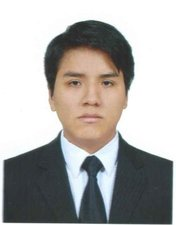
\includegraphics[width=0.6\columnwidth]{profile}
	\vspace{-7cm}
\end{figure}

\begin{flushright}\small
	Javier Huaman Adama \\
	\url{javier.adama@gmail}  \\
	(+51) 950450833
	\Sep
	\textbf{Dirección} \\
	Calle 3 de Mayo \\ % Address 1
	Mz. A Lt. 8 Urb. El Bosque \\ % Address 2
	Ate - Lima \\ % Address 3
\end{flushright}\normalsize
\framebreak

\CVItem{Febrero 2015 - Marzo 2017, Desarrollador Web, CAVASOFT SAC}\\
- Implementación de una solución tecnologica para el control de lavado de activos para Agentes de Aduana. Tecnologia usadas:\\
Spring MVC, Spring Security, iText, MongoDB, Git, Maven, Tomcat.\\\\
- Desarrollo de un software de asesor de comercio exterior para Agentes de Aduana. Tecnologia usadas:\\
Spring MVC, Spring Security, SQL Server 2012, Bazaar, Maven,Tomcat.\\\\
- Diseño de webservices para la generación de informe anual de registro de operaciones. Tecnologia usadas:\\
Python(módulos especializados).
\SmallSep

% Skills
\CVSection{Lenguajes}
\begin{multicols}{3}
\begin{compactitem}[\color{RoyalBlue}$\circ$]
	\item Java
	\item Python
	\item NodeJS
	\item Unix Shell
	\item Android
\end{compactitem}
\end{multicols}
\SmallSep

\CVItem{General}{
\begin{itemize}[noitemsep]
  \item Frameworks
  \begin{itemize}
    \item J2EE (JSP, JSTL, Servlet),
          JSF (Primefaces),
          Spring (MVC, Spring security),
          Maven, JUnit, Struts2, GAE (Google AppEngine),
          Flask, Django, Express.
  \end{itemize}
  \item Base de Datos
  \begin{itemize}
    \item MySQL (Intermedio), SQL Server 2012 (Intermedio), Oracle (Básico), JPA, Hibernate, JDBC.
  \end{itemize}
  \item Sistema Operativos
  \begin{itemize}
    \item Windows (7, 8), Linux (Debian, Ubuntu, CentOS, openSUSE).
  \end{itemize}
  \item Web
  \begin{itemize}
    \item HTML, CSS, Jquery, JSON, XML, Frameworks visuales (SemanticUI, Bootstrap), JS.
  \end{itemize}
  \item Repositorios
  \begin{itemize}
    \item Git, Bazaar, Subversion.
  \end{itemize}
  \item Herramientas
  \begin{itemize}
    \item Sublime Text, Eclipse (Mars, Luna), MySQL Worbench.
  \end{itemize}
\end{itemize}
}

\clearpage

\begin{figure}
	\hfill
	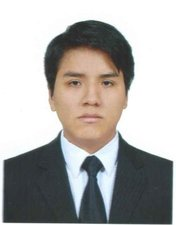
\includegraphics[width=0.6\columnwidth]{profile}
	\vspace{-7cm}
\end{figure}

\begin{flushright}\small
	Javier Huaman Adama \\
	\url{javier.adama@gmail}  \\
	(+51) 950450833
	\Sep
	\textbf{Dirección} \\
	Calle 3 de Mayo \\ % Address 1
	Mz. A Lt. 8 Urb. El Bosque \\ % Address 2
	Ate - Lima \\ % Address 3
\end{flushright}\normalsize
\framebreak

%----------------------------------------------------------------------------------------
% COMMUNICATION SKILLS
%----------------------------------------------------------------------------------------

\CVSection{Proyectos Personales/Educativos}

%------------------------------------------------

\CVItem{Sistema de Control de Correo Electronico}{
Software para la administración de diversas cuentas de correo electronico
\begin{itemize}[noitemsep]
  \item Tecnologia usadas:
  \begin{itemize}
    \item Java (Servlet, JSP, JSTL), MySQL, Maven, Git.
  \end{itemize}
\end{itemize}
}

%------------------------------------------------

\CVItem{Sistema de Reserva para un Cine}{
Se implemento un sistema con lenguaje Java que se alimenta de un web services
para los procesos de buscar cartelera, registrar una nueva reserva y buscar reserva.
\begin{itemize}[noitemsep]
  \item Tecnologia usadas:
  \begin{itemize}
    \item Java Web Service, Java (Servlet, JSP, JSTL), Tomcat, MySQL, Maven, Git.
  \end{itemize}
\end{itemize}
}

%------------------------------------------------

\CVItem{Sistema de control de máquina remoto}{
Se implementó un sistema para el control de máquinas desde un servidor de manera remota.
(Envío de archivos, apagar/encender/reiniciar máquina). Mediante sockets usando Java.
\begin{itemize}[noitemsep]
  \item Tecnologia usadas:
  \begin{itemize}
    \item Java sockets, Swing, Git.
  \end{itemize}
\end{itemize}
}

%------------------------------------------------

\CVItem{Sistema de Red Social}{
Se implementó un sistema en base de una red social.
\begin{itemize}[noitemsep]
  \item Tecnologia usadas:
  \begin{itemize}
    \item Primefaces, JSF, MySql, JPA, Maven, JUnit, Git.
  \end{itemize}
\end{itemize}
}

%------------------------------------------------

\CVItem{Examen en linea}{
Se implementó un sistema permite realizar examenes en linea.
\begin{itemize}[noitemsep]
  \item Tecnologia usadas:
  \begin{itemize}
    \item Primefaces, JSF, MySql, JPA, Maven, JUnit, Git.
  \end{itemize}
\end{itemize}
}

%------------------------------------------------

\Sep % Extra whitespace after the end of a major section


\CVSection{Cursos/Seminarios/Eventos}

%------------------------------------------------

\CVItem{2018, \textit{Hackatrix 2018}, Belatrix-BCP}

%------------------------------------------------

\CVItem{2016, \textit{Diplomado en Innovación e Integración Tecnológia}, CIBERTEC}

%------------------------------------------------

\CVItem{2014, \textit{Intercambio AIEP-Conferencias}, AIEP-Chile}


\CVSection{Referencias}

%------------------------------------------------

\CVItem{Profesional}{
\begin{itemize}[noitemsep]
  \item Github (\url{https://github.com/Hetaki})
  \item Launchpad (\url{https://launchpad.net/~jahanjp09})
  \item BitBucket (\url{https://bitbucket.org/JavierHuaman/})
  \item Udemy (\url{https://www.udemy.com/user/javier-antonio-huaman-adama/})
\end{itemize}
}

%------------------------------------------------

\CVItem{Social}{
\begin{itemize}[noitemsep]
  \item Linkedin (\url{https://www.linkedin.com/in/javierhuaman})
\end{itemize}
}


%%%%%%%%%%%%%%%%%%%%%%%%%%%%%%%%%%%%%
% End document
%%%%%%%%%%%%%%%%%%%%%%%%%%%%%%%%%%%%%
\end{document}